
\chapter{Przegląd badań na temat eksploracji danych sportowych oraz pojęcia podstawowe}

Rozdział tzw. state of the related research --- przegląd literatury naświetlający stan wiedzy na dany temat oraz pojecia zwiazane z tym co bedziecie wykorzystaywac

\textbf{Dodajcie jakis wstepny podrozdzial opisujace dokladniej wybrane zastosowania ML w analizie rozgrywek sportowych - glownie czym sie zajmuja badacze, jakie problemy teoretyczne i praktyczne badali + jakie byly typy rozgrywek - to w jakis sposob robiliscie iles miesiecy temu w ramach tzw. przegladu na google docs}
Na koncu musiecie cos powiedziec ze Wasze plany systemu wiaza sie z koniecznoscia odwolanie sie do repozytoriów danych, pozyskania ich oraz wstepnego przetworzenia - dlatego dalej 

\section{Bazy danych i API}
Opisy relacyjnych baz danych i Web API
\section{Wstępne przetwarzanie i wizualizacja danych}

\noindent 

Jednym z kluczowych aspektów mocno wpływających na powodzenie każdego projektu związanego z uczeniem maszynowym jest stworzenie odpowiedniego zbioru cech (\english{features}) na podstawie poprawnie przygotowanych danych. W kontekście uczenia maszynowego, cecha to indywidualna, mierzalna własność lub charakterystyka pewnego obserwowanego zjawiska~\cite{Wiki:Feature}. W przypadku modelu przewidującego wyniki meczów piłkarskich, przykładem cechy może być liczba żółtych kartek uzyskanych przez drużynę gospodarzy w ostatnim meczu lub średni procent posiadania piłki drużyny gości w meczach obecnego sezonu.

Metody zbioru danych są bardzo często automatyzowane i pozbawione ścisłej kontroli, stąd mogą one zawierać różnego rodzaju błędy, takie jak wartości spoza zakresu (np. wiek: -20), niemożliwe kombinacje wartości (płeć: mężczyzna, w ciąży: tak) lub pominięte atrybuty dla niektórych rekordów. Ważne jest, aby takie błędy wychwycić już na etapie wstępnego przetwarzania i nie dopuścić ich do danych wejściowych algorytmów. Pomocna może się tutaj okazać wizualizacja dokonana w celu bliższego zapoznania się z danymi. Dla atrybutów można wizualizować ich wartości przy pomocy histogramów lub wypisywać ich podstawowe statystyki (m.in. średnie, mediany, wartości minimalne, maksymalne) w celu weryfikacji poprawności ich zakresów i typów.

System będzie w stanie nauczyć się przewidywać wyniki tylko mając do dyspozycji jak najwięcej znaczących cech i jak najmniej tych mało znaczących. Zgodnie z popularnym angielskim zwrotem w obszarze przetwarzania informacji-  \definicja{śmieci na wejściu – śmieci na wyjściu} (\english{Garbage In, Garbage Out, GIGO}), nawet skuteczny i poprawnie działający program w przypadku otrzymania na wejściu błędnych danych, da na wyjściu niepoprawne oraz mało użyteczne wyniki, stąd tak ważne jest uprzednie przygotowanie danych.

Wstępne przetwarzanie (\english{preprocessing}) w naszym systemie składa się z jednorazowego dokonania wizualizacji posiadanych przez nas danych (która będzie szczegółowo przedstawiona w późniejszym rozdziale) w celu pogłębienia wiedzy na ich temat i wyszukania potencjalnych braków lub błędów. Następnym zadaniem, wykonywanym każdorazowo przy tworzeniu zbioru danych, którego przeznaczeniem jest użycie podczas testowania różnego rodzaju algorytmów, jest pobranie interesujących danych z bazy, przetworzenie ich, czyli poradzenie sobie z m.in. wartościami pustymi i stworzenie na ich podstawie zbioru cech reprezentujących każdy rekord (w przypadku naszego systemu jest to pojedynczy mecz). 

Wynikiem etapu wstępnego przetwarzania jest tzw. zbiór treningowy (\english{training set}), którego znaczenie zostanie przybliżone w podrozdziale traktującym o algorytmach uczenia maszynowego.

\section{Sposób oceny wyników predykcji}

Różne algorytmy dają różne wyniki. Przy pomocy jednych uzyskujemy tylko konkretną klasę, do której przynależy konkretne wejście, a inne przyporządkowują rozkład prawdopodobieństwa możliwych wyników klasyfikacji. W naszym przypadku, mamy do czynienia z obiema sytuacjami. Podczas doboru sposobu oceny naszych algorytmów głównym celem było dobranie takich miar, aby móc wzajemnie porównywać zastosowane algorytmy i na tej podstawie dobrać najlepsze podejście. Ocena jakości naszych rozwiązań opierała się zatem na policzeniu dokładności (\english{accuracy}) na zbiorze testowym (wynoszącym 10\% całego zbioru danych), macierzy pomyłek oraz wynikające z nich miary takie jak: precision, recall oraz F-score, które wyznaczyliśmy przy użyciu średniej typu „macro” (oblicza metryki dla każdej etykiety, a następnie wyznacza ich nieważoną średnią. Metoda ta nie uwzględnia niezbalansowania danych).

\begin{center}
\renewcommand{\arraystretch}{1.5}
\begin{tabular}{|c|c|c|c|c|}
   \cline{3-5} 
   \multicolumn{1}{c}{} & & \multicolumn{3}{c|}{Predicted} \\ \cline{3-5}
   \multicolumn{1}{c}{} & & Draw & HomeWin & AwayWin \\ \hline
   
   {Observed}
   & Draw & .. & .. & ..  \\ \cline{2-5}
   & HomeWin & .. & .. & ..  \\ \cline{2-5}
   & AwayWin & .. & .. & .. \\ \hline
\end{tabular}
\end{center}
Dodatkowo przetestowaliśmy nasze algorytmy w sposób, w którym dane wejściowe podzieliliśmy na bloki następujące po sobie. Następnie wyuczyliśmy nasz algorytm na pierwszym bloku i testowaliśmy jego działanie na mniejszym bloku, który w zbiorze danych wstępował zaraz po bloku uczącym. Kolejno do dotychczasowego zbioru uczącego dołożyliśmy dane z poprzedniego bloku testowego i na podstawie nowego zbioru znów dokonaliśmy uczenia maszynowego by następnie dokonać ewaluacji na kolejnym fragmencie zbioru testowego. Proces ten powtarzaliśmy, aż do wykorzystania wszystkich dostępnych i przygotowanych danych.
\newpage

\section{Algorytmy uczenia maszynowego}
opisy teoretyczne wykorzystywanych algorytmów
Przegląd literatury naświetlający stan wiedzy na dany temat obejmuje rozdziały pisane na podstawie
literatury, której wykaz zamieszczany jest w części pracy pt.~\emph{Literatura} (lub inaczej \emph{Bibliografia},
\emph{Piśmiennictwo}). W tekście pracy muszą wystąpić odwołania do wszystkich pozycji zamieszczonych w
wykazie literatury. \textbf{Nie należy odnośników do literatury umieszczać w stopce strony.} Student jest
bezwzględnie zobowiązany do wskazywania źródeł pochodzenia informacji przedstawianych w pracy,
dotyczy to również rysunków, tabel, fragmentów kodu źródłowego programów itd. Należy także podać
adresy stron internetowych w przypadku źródeł pochodzących z Internetu. 


\subsection{Metoda Wektorów Wspierających - SVM}
\definicja{Metoda wektorów wspierających - nośnych} (\english{Support Vector Machine, SVM}), jest to nadzorowana technika uczenia maszynowego wykorzystywana do zadań klasyfikacji oraz regresji. Technika ta została opracowana w laboratorium AT\&T Bell poprzez Vladimira Naumovicha Vapnika wraz z współpracownikami (Boser i in., 1992, Guyon i in., 1993, Vapnik i in., 1997). \cite{Wiki:SVM}. Głównym założeniem tej metody jest wyznaczenie hiperpłaszczyzny, która ma za zadanie rozdzielić przy pomocy maksymalnego marginesu przykłady należące do różnych klas. W przypadku występowania więcej niż dwóch klas, metoda ta wykorzystuję technikę \definicja{OvR} (\english{One-vs-Rest}), która polega na szkoleniu jednego klasyfikatora na klasę, z próbkami z tej klasy jako pozytywne próbki, a inne próbki jako negatywy. Formalnie problem klasyfikacji przedstawia się następująco \cite{Prezentacja:SVM2}: 
\begin{itemize}
    \item W przestrzeni danych (ang. measurement space) $\omega$ znajdują się wektory danych x stanowiące próbkę uczącą D, należące do dwóch klas\\
    \begin{equation}
D = \big\{(x_{i}, c_{i}) | x_{i} \in R^{p}, c_{i} \in \{-1, 1\}\big\}_{i=1}^{N}
    \end{equation}
    \item Szukamy klasyfikatora pozwalającego na podział całej przestrzeni $\omega$ na dwa rozłączne obszary odpowiadającej klasom {1,-1} oraz pozwalającego jak najlepiej klasyfikować nowe obiekty x do klas
    \item Podejście opiera się na znalezieniu tzw. granicy decyzyjnej między klasami → g( x )
\end{itemize}
Dodatkowo dwie klasy są liniowo separowalne, jeśli istnieje hiperpłaszczyzna H postaci: \[g(x) = w^Tx + b\] przyjmująca wartości: 

\[
    \begin{cases}
            g(x_{i}) > 0,& x_{i} \in 1 \\
            g(x_{i}) < 0,& x_{i} \in -1
    \end{cases}
\]
\\

Linia granicy decyzyjnej nie tylko oddziela dwie klasy, ale także pozostaje jak najdalej od najbliższych instancji. Jak pokazano na rysunku \ref{SVM-margines} problemem poza znalezieniem $B_{2}$ jest również znalezienie szerokości wspomnianej granicy. Niestety nie ma na to idealnego rozwiązania i konieczne jest wybranie cech, które są bardziej odpowiednie dla naszego problemu. Szerszy margines to lepsze własności generalizacji, mniejsza podatność na
ewentualne przeuczenie (\english{overfitting}), a z kolei wykorzystanie wąskiego marginesu skutkuje radykalną zmianą klasyfikacji przy małej zmianie granicy. Jednak ze względu na oszacowanie górnej granicy błędu ze względu na błąd uczący częściej wybiera się jak najszerszy margines w celu lepszego uogólniania w bardziej skomplikowanych modelach.

\begin{figure}[h] 
        \centering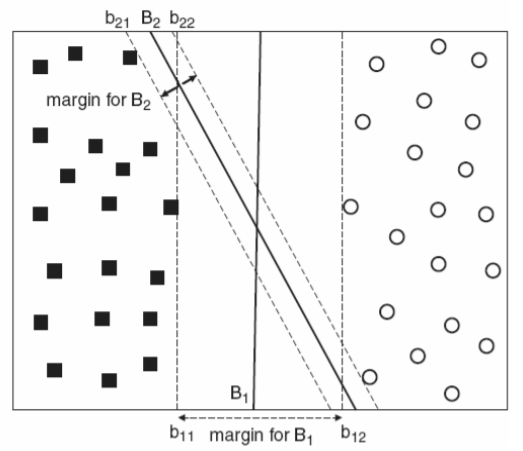
\includegraphics[width=6cm,height=6cm]{figures/SVM-margin.png}
        \caption{Margines granicy decyzyjnej}\label{SVM-margines}
\end{figure}
Konsekwentnie, problem maszyn wektorów nośnych sprowadza się do poszukiwania maksymalnego marginesu klasyfikacji: $w x + b = 0$ gdzie \definicja{w} oraz \definicja{b} są parametrami modelu.
\[
y = 
    \begin{cases}
            1,&  wx+b > 0\\
            -1,& wx+b < 0
    \end{cases}
\]
Dodatkowo parametry granicy wyznacza się tak, aby maksymalne marginesy (margines to odległość między \definicja{bi1} oraz \definicja{bi2}) \definicja{bi1} i \definicja{bi2} były miejscem geometrycznym punktów \definicja{x} spełniających warunki \ref{SVM-marginesEq}:
\[
    \begin{cases}
            bi1,&  wx+b = 1\\
            bi2,& wx+b= -1
    \end{cases}
\]
\begin{figure}[h] 
        \centering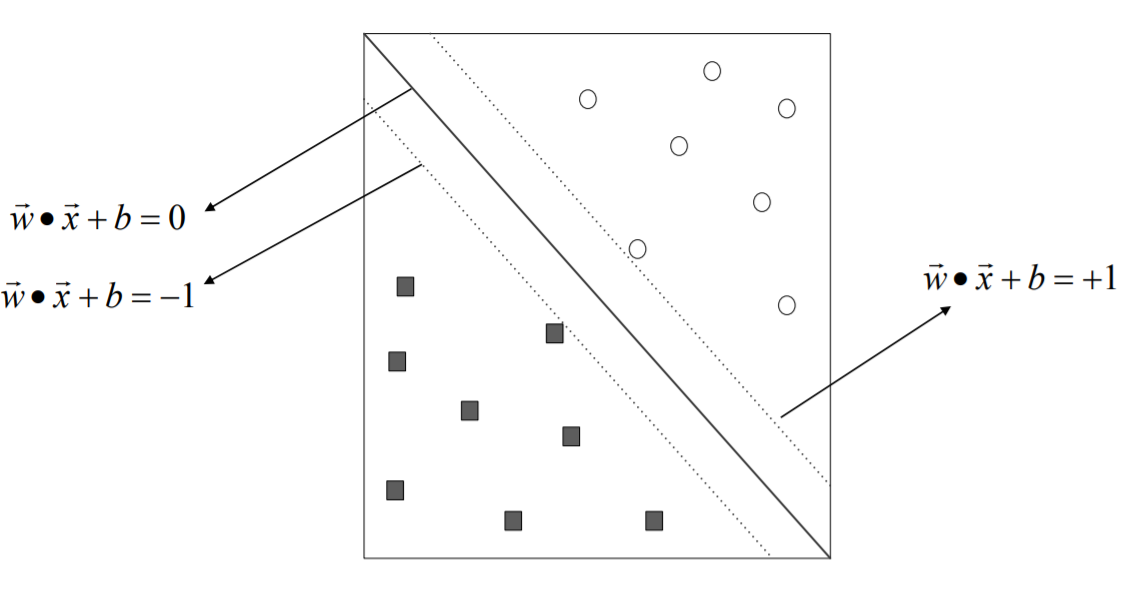
\includegraphics[width=14cm,height=6cm]{figures/SVM-marginEq.png}
        \caption{Wyznaczanie marginesu granicy decyzyjnej}\label{SVM-marginesEq}
\end{figure}
\\
Tak więc problem ten sprowadza się do optymalizacji kwadratowej z liniowymi ograniczeniami (uogólnione zadanie optymalizacji). 
Czasami jednak mamy do czynienia z sytuacją podczas której nie mamy możliwości w pełni liniowej separacji klas. W takiej sytuacji wykorzystuje się zmienne osłabiające \definicja{$\xi_{i} \ge 0$}, które dobiera się dla każdego przykładu uczącego. Jej wartość zmniejsza margines separacji. Jeżeli $0 \le \xi_{i} \le 1$, to punkt danych $(xi,di)$ leży wewnątrz strefy separacji, ale po właściwej stronie, a w sytuacji gdy $\xi_{i} \ge 1$, to punkt leży po niewłaściwej stronie hiperpłaszczyzny i nastąpi błąd klasyfikacji. 
\[
    \begin{cases}
            bi1,&  wx+b = 1 - \xi\\
            bi2,& wx+b= -1 + \xi
    \end{cases}
\]
Również tutaj występuje konflikt doboru marginesu. Szeroki margines to dużo błędów i odwrotnie. Kończąc rozważania dotyczące liniowej maszyny wektorów nośnych, nasz problem znalezienia granicy decyzyjnej sprowadza się do minimalizacji wyrażenia:
\[
L(w) = \frac{\|\vec{w}\|}{2} + C\big(\sum_{i=1}^{N}\xi_{i}^{k}\big)
\]
z ograniczeniami:
\[
f(\vec{x_{i}}) = 
    \begin{cases}
            1 &  \text{if}\ \vec{w} \bullet \vec{x_{i}}+b \ge 1 - \xi_{i}\\
            -1 &  \text{if}\ \vec{w} \bullet \vec{x_{i}}+b \le 1 + \xi_{i}
    \end{cases}
\]
gdzie parametr \definicja{C} to ocena straty związanej z każdym błędnie klasyfikowanym punktem dla którego $\xi > 0$. Problem ten to problem dualny i istnieją techniki pozwalające na jego rozwiązanie.

Dodatkowym problemem w tej metodzie jest fakt, że najczęściej klasy nie są liniowo separowane. Jednym ze sposobów na poradzenie sobie z tym problemem jest transformowanie, projekcja danych wejściowych do przestrzeni o większej liczbie wymiarów, w której dane, z dużym prawdopodobieństwem będą separowane liniowo. Funkcja decyzyjna po przekształceniu ma się następująco:
\[
g(x) = w\varphi(x) + b
\]
Problem ten jest trudny obliczeniowo do wykonania, lecz można sobie z nim poradzić za pomocą kerneli, funkcji jądrowych. Funkcje te wywodzą się z badań liniowych przestrzeni wektorowych, przestrzeni Hilberta, Banacha. Dzięki nim można wyznaczyć potrzebne parametry do rozwiązania naszego problemu. Najczęściej stosowane jądra w metodzie maszyn wektorów nośnych to: Gaussowskie, wielomianowe i sigmoidalne. Dzięki nim, nie musimy znać funkcji transformacji, a jedynie funkcję kernela co pozwala nam na pracę w nowej przestrzeni. 

Można zauważyć, że metoda SVM jest silną metodą pozwalającą na rozwiązywanie problemów klasyfikacji w wielowymiarowej przestrzeni danych. Dzięki niej można skutecznie uogólniać nowe przykłady i przydzielać im odpowiednie klasy zdefiniowane dla konkretnego problemu.

\subsection{Sztuczne Sieci Neuronowe - SNN}

\definicja{Sztuczna sieć neuronowa} ogólna nazwa struktur matematycznych i ich programowych lub sprzętowych modeli, realizujących obliczenia lub przetwarzanie sygnałów poprzez rzędy elementów przetwarzających, zwanych sztucznymi neuronami, wykonujących pewną podstawową operację na swoim wejściu. Oryginalną inspiracją takiej struktury była budowa naturalnych neuronów, łączących je synaps, oraz układów nerwowych, w szczególności mózgu \cite{Wiki:SNN}. Sztuczne sieci neuronowe charakteryzują się tym, że mają zdolność do odwzorowania różnych zależności pomiędzy sygnałami wejściowymi i wyjściowymi. Sztuczna sieć neuronowa składa się z wielu połączonych neuronów, a kady neuron można interpretować jako pewna kombinacja matematyczna cech wejściowych wraz z przypisanymi im wagami. Wyjście neuronu to pewna funkcja matematyczna, która przekształca daną kombinację danych wejściowych i przekazuje taki wynik na swoje wyjście. Graficzna reprezentacja takiego neuronu ma się następująco \cite{Prezentacja:SNN} --- \textbf{to jest także ze skryptu KKJS}:
\begin{figure}[h] 
        \centering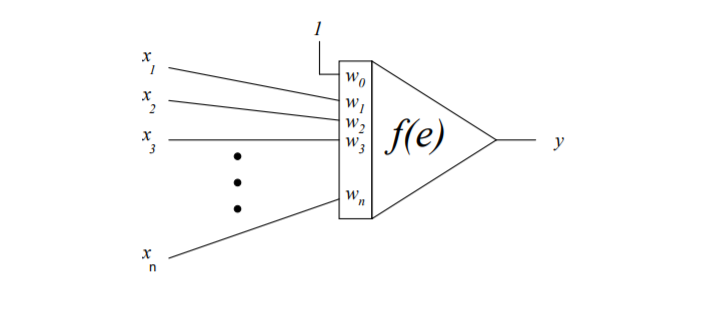
\includegraphics[width=12cm,height=6cm]{figures/SNN.png}
        \caption{Sztuczny neuron}\label{SVM-neuron}
\end{figure}

Podstawowe elementy składowe: 
\begin{itemize}
    \item n wejść neuronu wraz z wagami $w_{i}$ (wektor wag w i wektor sygnałów wejściowych x)
    \item jeden sygnał wyjściowy y
    \item pobudzenie e neuronu jako suma ważona sygnałów wejściowych
pomniejszona o próg $\Theta$
\[
e = \sum_{i=1}^{N} w_{i} x_{i} - \Theta = w^{T} x - \Theta
\]
wprowadźmy wagę $w_{0}= \Theta$, podłączonej do stałego sygnału $x_{0} = 1$;
wówczas: 
\[
e = \sum_{i=0}^{N} w_{i} x_{i}  = w^{T} x
\]
\item funkcja aktywacji (przejścia):
\[
y = f(e)
\]
\end{itemize}
Kluczowe znaczenie dla działania neuronu ma funkcja aktywacji. Mamy do wyboru liniową funkcję lub nielinową (ciągła i nieciągła, unipolarna i bipolarna).

W literaturze wyróżnia się dwa ogólne typy sieci neuronowych i są to: jednokierunkowe SNN oraz rekurencjne SNN (sieci ze sprzężeniami zwrotnymi np. sieć Hopfielda albo sieci uczenia się przez współzawodnictwo).
Sieci jednokierunkowe to sieci o jednym kierunku przepływu sygnałów. Szczególnym przypadkiem architektury jednokierunkowej jest sieć warstwowa, reprezentująca zdecydowanie najpopularniejszą topologię.
\begin{figure}[h] 
        \centering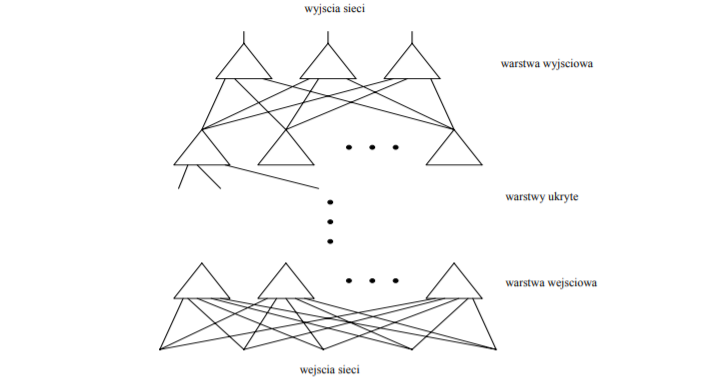
\includegraphics[width=12cm,height=6cm]{figures/ArchitekturaSNN.png}
        \caption{Sieć warstwowa jednokierunkowa}\label{SVM-neuron}
\end{figure}

Zasady łączenia neuronów między sobą:
\begin{itemize}
    \item każdy neuron z każdym,
    \item połączenia między kolejnymi warstwami w sieciach warstwowych,
    \item tylko z pewną grupą neuronów, najczęściej z tzw. sąsiedztwem
\end{itemize}

W celu uzyskania wyników wykorzystuje się \definicja{uczenie nadzorowane}. Dany jest zbiór przykładów uczących składający się z par wejście-wyjście $(x_{j}, z_{j})$, gdzie $z_{j}$ jest pożądaną odpowiedzią sieci na sygnały wejściowe $x_{j} (j=1,..m)$. Zadaniem sieci jest nauczyć się możliwie jak najdokładniej funkcji przybliżającej powiązanie wejścia z wyjściem. Odległość pomiędzy rzeczywistą a pożądaną odpowiedzią sieci jest
miarą błędu używaną do korekcji wag sieci. Typowym przykładem jest uczenie sieci wielowarstwowej algorytmem wstecznej propagacji błędu; każdy neuron lokalnie zmniejsza swój błąd stosując metodę spadku gradientu.

W celu uczenia sieci neuronowych wykorzystuje się kilka reguł i są nimi między innymi: \definicja{reguła Widrowa-Hoffa} oraz \definicja{reguła delta}. Pierwsza z nich dotyczy uczenia nadzorowanego sieci jednokierunkowych, gdzie minimalizuje się błąd pomiędzy pożądaną a aktualną odpowiedzią. 
\[
\delta^{j} = z^{j} - y^{j} = z^{j} - w^{T}x^{j}
\]

Korekta wag jest następująca \cite{Widrow}:
\begin{equation}
\label{eqn:delta}
\delta w_{i} = \eta \delta^{j} x^{j}_{i}
\end{equation}
Reguła delta z kolei obowiązuje dla neuronów z ciągłymi funkcjami aktywacji i nadzorowanego trybu uczenia. Regułę delta wyprowadza się jako wynik minimalizacji kryterium błędu średnio-kwadratowego Q.
\[
Q = \frac{1}{2}\sum_{j=1}^{N} \big( z^{j} - y^{j}\big)^{2} = \sum_{j}^{N}Q^{j}, Q^{j} = \frac{1}{2}(\delta^{j})^{2}
\]

Korekta wag:
\[
\delta w_{i} = \eta \delta^{j} (1 - y^{j}) f'(e^{j}) x^{j}_{i}
\]
gdzie $f'()$ oznacza pochodną funkcji aktywacji. Stosowana jest do uczenia wielowarstwowych sieci neuronowych wraz z algorytmem wstecznej propagacji błędów \cite{Rumelhart}. Sieci charakterystyczne cechują się pewnymi właściwościami \cite{Mitchell}:
\begin{itemize}
    \item Przykłady uczące opisane są przez pary atrybut-wartość (na ogół
zdefiniowanych na skalach liczbowych,
    \item Przybliżana funkcja może mieć wartości dyskretne lub rzeczywiste;
może być także wektorem wartości,
 \item Dane mogą zawierać błędy lub podlegać zniekształceniu. SSN są
odporne na różnego rodzaju uszkodzenia danych, 
    \item Akceptowalny jest długi czas uczenia sieci,
    \item Akceptacja dla potencjalnie dużej liczby parametrów algorytmu,
które wymagają dostrojenia metodami eksperymentalnymi,
    \item Zadanie nie wymaga rozumienia przez człowieka funkcji
nauczonej przez SNN - trudności z interpretacją wiedzy nabytej
przez sieć (rozwijający się w tym momencie sektor uczenia maszynowego XAI - \english{explainable artificial intelligence}).
\end{itemize}

Jednak kluczowym konceptem sprawiającym, że sztuczne sieci neuronowe są tak popularne i oferujące wiele możliwości jest wsteczna propagacja błędów, czyli sposób w jaki sieć nabywa umiejętności generalizowania danych i przyporządkowywania odpowiednich wartości. Błąd k-tego neuronu w l-tej warstwie jest równy sumie błędów popełnionych przez neurony (p) z warstwy l+1-szej ważonych po wagach $w_{k(p,l+1)}$ łączących ten neuron z neuronami tej warstwy \cite{Prezentacja:SNN}: 

\[
\delta_{(k,l)}^{j} = \sum_{p=1}^{N_{l+1}} W^{j}_{k(p, l+1)} \delta_{(p,l+1)}^{j}
\]

Na podstawie wstecznej propagacji błędów, sieci neuronowe modyfikują wagi dla każdego neuronu dopowiadające danym wejściowym w celu minimalizacji funkcji nazywanej \definicja{funkcją straty}.

Wartości początkowe wag muszą być zainicjowane przed przystąpieniem do procesu uczenia i zazwyczaj dokonuje się tego w sposób losowy lub na podstawie pewnego rozkładu prawdopodobieństwa. Kluczowym czynnikiem do prędkości oraz jakości otrzymywanych wyników jest współczynnik $\eta$, który już mogliśmy zauważyć w równaniu \ref{eqn:delta}. Decyduje on o wpływie błędu popełnianego przez neuron na korektę wartości wag. Właściwy dobór ma kluczowe znaczenie dla prędkości zbieżności algorytmu, a jego zbyt mała wartość spowalnia proces uczenia i zwiększa ryzyko
wpadnięcia w pułapkę lokalnego minimum \cite{Prezentacja:SNN}. 

Niestety sieć neuronowa jest trudnym narzędziem i występuję w niej problem doboru wielkości warstw ukrytych, który do teraz jest problemem otwartym. 
Nie istnieje jednoznaczna reguła określająca optymalny rozmiar danej warstwy oraz ilości warstw w danej sieci przy danym zbiorze uczącym. Zbyt mała wielkość warstw czyni sieć niezdolną do adaptacji do
zadanego zbioru przykładów co skutkuje, że w trakcie uczenia błąd
średnio-kwadratowy utrzymuje dużą wartość. Zbyt duże warstwy z kolei mają problem z przeuczaniem (nauka konkretnych wartości danych wejściowych, a nie ogólnego konceptu, zarysu) \cite{Prezentacja:SNN}.

Od początku historii SNN do teraz powstało mnóstwo konceptów, pomysłów, sztuczek i schematów które zapewniają lepsze generalizowanie, szybsze zbieganie do minimum, które nie sposób zebrać i opisać w jednym miejscu. Wiele technik zapewniło uczenie bardzo dużych sieci neuronowych zapewniających stabilne gradienty (jednym z problemów podczas nauki SNN jest niestabilność gradientów, które zanikały wraz z postępem algorytmu lub wręcz eksplodowały do bardzo dużych wartości) \cite{gradient}. Powstało również wiele funkcji aktywacji oraz sposobów inicjalizacji początkowych wag sieci.

